\scanpage{155}
% archive sheet number: 154
qu'on a un \deleted{\unsure{Module}} ``vectoriel $\ell$-adique'' [ou ``Module $\ell$-adique''\unsure{)|]} \uline{attaché \unsure{à|:} $A$} si on a un élément de
\[
\unsure{\mathcal V|\mathscr V}((A_i))=\underset{\longrightarrow}{\operatorname{Pseudolim}}\mathcal V(A_i).
\]
Si $A$ est normal \inserted{(p.ex)} il lui est attaché \deleted{\unsure{une}} \inserted{\unsure{canoniquement}} [pour tt pt géométrique $\xi$ de $S$] une ss-algèbre de Lie $\mathfrak g_\xi$ de $\mathfrak{gl}(V_\xi)$.

D'ailleurs, l'image de $\pi_1(S,\xi)\unsure{\text{---}|\longrightarrow}\operatorname{Aut}(V_\xi)$ définit un autre ss-groupe analytique, donc une algèbre de Lie $\mathfrak g'_\xi\unsure{\ell|l|)}\unsure{\subset|\subseteq}\mathfrak g_\xi$. La formation de $\mathfrak g_\xi$ est \deleted{compatible} \uline{insensible} par \uline{extension \inserted{(dominante)} de la base}, contrairement à celle de $\mathfrak g'_\xi$ [$\mathfrak g'_\xi$ \uline{diminue} quand $(S,\xi)$ est remplacé \unsure{par} $(S',\xi')$ au dessus,].
\margin{\figure{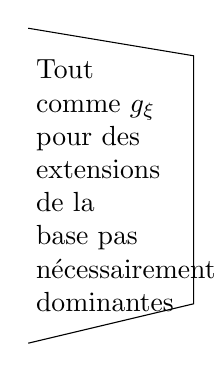
\begin{tikzpicture}\node[align=left,text width=1.9cm,inner sep=0pt] at (0,0) {Tout comme $\mathfrak g_\xi$ pour des extensions de la base pas nécessairement dominantes};\draw (-1.05,2)--(1.05,1.65)--(1.05,-1.5)--(-1.05,-2);\end{tikzpicture}}}
\inserted{Si d'ailleurs $A$ est de type fini \unsure{sur $\mathbb Z$|bien sûr}, on a évidemment $\mathfrak g'_\xi=\mathfrak g_\xi$.}

On constate facilement que [dans le cas général d'un système $(S_i)$ ...] \deleted{\unsure{en faisant}} le choix des \deleted{\unsure{les}} ``\unsure{classes de Chemins|classes de chemins}'' de $\xi$ à $\xi'$ \deleted{\unsure{type}} (\unsure{p\textsuperscript{ce} qu'on a dit|v\textsuperscript{ce} qu'on a dit|vu ce qu'on a dit}) définit
